% Options for packages loaded elsewhere
% Options for packages loaded elsewhere
\PassOptionsToPackage{unicode}{hyperref}
\PassOptionsToPackage{hyphens}{url}
\PassOptionsToPackage{dvipsnames,svgnames,x11names}{xcolor}
%
\documentclass[
  letterpaper,
  DIV=11,
  numbers=noendperiod]{scrartcl}
\usepackage{xcolor}
\usepackage{amsmath,amssymb}
\setcounter{secnumdepth}{5}
\usepackage{iftex}
\ifPDFTeX
  \usepackage[T1]{fontenc}
  \usepackage[utf8]{inputenc}
  \usepackage{textcomp} % provide euro and other symbols
\else % if luatex or xetex
  \usepackage{unicode-math} % this also loads fontspec
  \defaultfontfeatures{Scale=MatchLowercase}
  \defaultfontfeatures[\rmfamily]{Ligatures=TeX,Scale=1}
\fi
\usepackage{lmodern}
\ifPDFTeX\else
  % xetex/luatex font selection
\fi
% Use upquote if available, for straight quotes in verbatim environments
\IfFileExists{upquote.sty}{\usepackage{upquote}}{}
\IfFileExists{microtype.sty}{% use microtype if available
  \usepackage[]{microtype}
  \UseMicrotypeSet[protrusion]{basicmath} % disable protrusion for tt fonts
}{}
\makeatletter
\@ifundefined{KOMAClassName}{% if non-KOMA class
  \IfFileExists{parskip.sty}{%
    \usepackage{parskip}
  }{% else
    \setlength{\parindent}{0pt}
    \setlength{\parskip}{6pt plus 2pt minus 1pt}}
}{% if KOMA class
  \KOMAoptions{parskip=half}}
\makeatother
% Make \paragraph and \subparagraph free-standing
\makeatletter
\ifx\paragraph\undefined\else
  \let\oldparagraph\paragraph
  \renewcommand{\paragraph}{
    \@ifstar
      \xxxParagraphStar
      \xxxParagraphNoStar
  }
  \newcommand{\xxxParagraphStar}[1]{\oldparagraph*{#1}\mbox{}}
  \newcommand{\xxxParagraphNoStar}[1]{\oldparagraph{#1}\mbox{}}
\fi
\ifx\subparagraph\undefined\else
  \let\oldsubparagraph\subparagraph
  \renewcommand{\subparagraph}{
    \@ifstar
      \xxxSubParagraphStar
      \xxxSubParagraphNoStar
  }
  \newcommand{\xxxSubParagraphStar}[1]{\oldsubparagraph*{#1}\mbox{}}
  \newcommand{\xxxSubParagraphNoStar}[1]{\oldsubparagraph{#1}\mbox{}}
\fi
\makeatother

\usepackage{color}
\usepackage{fancyvrb}
\newcommand{\VerbBar}{|}
\newcommand{\VERB}{\Verb[commandchars=\\\{\}]}
\DefineVerbatimEnvironment{Highlighting}{Verbatim}{commandchars=\\\{\}}
% Add ',fontsize=\small' for more characters per line
\usepackage{framed}
\definecolor{shadecolor}{RGB}{241,243,245}
\newenvironment{Shaded}{\begin{snugshade}}{\end{snugshade}}
\newcommand{\AlertTok}[1]{\textcolor[rgb]{0.68,0.00,0.00}{#1}}
\newcommand{\AnnotationTok}[1]{\textcolor[rgb]{0.37,0.37,0.37}{#1}}
\newcommand{\AttributeTok}[1]{\textcolor[rgb]{0.40,0.45,0.13}{#1}}
\newcommand{\BaseNTok}[1]{\textcolor[rgb]{0.68,0.00,0.00}{#1}}
\newcommand{\BuiltInTok}[1]{\textcolor[rgb]{0.00,0.23,0.31}{#1}}
\newcommand{\CharTok}[1]{\textcolor[rgb]{0.13,0.47,0.30}{#1}}
\newcommand{\CommentTok}[1]{\textcolor[rgb]{0.37,0.37,0.37}{#1}}
\newcommand{\CommentVarTok}[1]{\textcolor[rgb]{0.37,0.37,0.37}{\textit{#1}}}
\newcommand{\ConstantTok}[1]{\textcolor[rgb]{0.56,0.35,0.01}{#1}}
\newcommand{\ControlFlowTok}[1]{\textcolor[rgb]{0.00,0.23,0.31}{\textbf{#1}}}
\newcommand{\DataTypeTok}[1]{\textcolor[rgb]{0.68,0.00,0.00}{#1}}
\newcommand{\DecValTok}[1]{\textcolor[rgb]{0.68,0.00,0.00}{#1}}
\newcommand{\DocumentationTok}[1]{\textcolor[rgb]{0.37,0.37,0.37}{\textit{#1}}}
\newcommand{\ErrorTok}[1]{\textcolor[rgb]{0.68,0.00,0.00}{#1}}
\newcommand{\ExtensionTok}[1]{\textcolor[rgb]{0.00,0.23,0.31}{#1}}
\newcommand{\FloatTok}[1]{\textcolor[rgb]{0.68,0.00,0.00}{#1}}
\newcommand{\FunctionTok}[1]{\textcolor[rgb]{0.28,0.35,0.67}{#1}}
\newcommand{\ImportTok}[1]{\textcolor[rgb]{0.00,0.46,0.62}{#1}}
\newcommand{\InformationTok}[1]{\textcolor[rgb]{0.37,0.37,0.37}{#1}}
\newcommand{\KeywordTok}[1]{\textcolor[rgb]{0.00,0.23,0.31}{\textbf{#1}}}
\newcommand{\NormalTok}[1]{\textcolor[rgb]{0.00,0.23,0.31}{#1}}
\newcommand{\OperatorTok}[1]{\textcolor[rgb]{0.37,0.37,0.37}{#1}}
\newcommand{\OtherTok}[1]{\textcolor[rgb]{0.00,0.23,0.31}{#1}}
\newcommand{\PreprocessorTok}[1]{\textcolor[rgb]{0.68,0.00,0.00}{#1}}
\newcommand{\RegionMarkerTok}[1]{\textcolor[rgb]{0.00,0.23,0.31}{#1}}
\newcommand{\SpecialCharTok}[1]{\textcolor[rgb]{0.37,0.37,0.37}{#1}}
\newcommand{\SpecialStringTok}[1]{\textcolor[rgb]{0.13,0.47,0.30}{#1}}
\newcommand{\StringTok}[1]{\textcolor[rgb]{0.13,0.47,0.30}{#1}}
\newcommand{\VariableTok}[1]{\textcolor[rgb]{0.07,0.07,0.07}{#1}}
\newcommand{\VerbatimStringTok}[1]{\textcolor[rgb]{0.13,0.47,0.30}{#1}}
\newcommand{\WarningTok}[1]{\textcolor[rgb]{0.37,0.37,0.37}{\textit{#1}}}

\usepackage{longtable,booktabs,array}
\usepackage{calc} % for calculating minipage widths
% Correct order of tables after \paragraph or \subparagraph
\usepackage{etoolbox}
\makeatletter
\patchcmd\longtable{\par}{\if@noskipsec\mbox{}\fi\par}{}{}
\makeatother
% Allow footnotes in longtable head/foot
\IfFileExists{footnotehyper.sty}{\usepackage{footnotehyper}}{\usepackage{footnote}}
\makesavenoteenv{longtable}
\usepackage{graphicx}
\makeatletter
\newsavebox\pandoc@box
\newcommand*\pandocbounded[1]{% scales image to fit in text height/width
  \sbox\pandoc@box{#1}%
  \Gscale@div\@tempa{\textheight}{\dimexpr\ht\pandoc@box+\dp\pandoc@box\relax}%
  \Gscale@div\@tempb{\linewidth}{\wd\pandoc@box}%
  \ifdim\@tempb\p@<\@tempa\p@\let\@tempa\@tempb\fi% select the smaller of both
  \ifdim\@tempa\p@<\p@\scalebox{\@tempa}{\usebox\pandoc@box}%
  \else\usebox{\pandoc@box}%
  \fi%
}
% Set default figure placement to htbp
\def\fps@figure{htbp}
\makeatother


% definitions for citeproc citations
\NewDocumentCommand\citeproctext{}{}
\NewDocumentCommand\citeproc{mm}{%
  \begingroup\def\citeproctext{#2}\cite{#1}\endgroup}
\makeatletter
 % allow citations to break across lines
 \let\@cite@ofmt\@firstofone
 % avoid brackets around text for \cite:
 \def\@biblabel#1{}
 \def\@cite#1#2{{#1\if@tempswa , #2\fi}}
\makeatother
\newlength{\cslhangindent}
\setlength{\cslhangindent}{1.5em}
\newlength{\csllabelwidth}
\setlength{\csllabelwidth}{3em}
\newenvironment{CSLReferences}[2] % #1 hanging-indent, #2 entry-spacing
 {\begin{list}{}{%
  \setlength{\itemindent}{0pt}
  \setlength{\leftmargin}{0pt}
  \setlength{\parsep}{0pt}
  % turn on hanging indent if param 1 is 1
  \ifodd #1
   \setlength{\leftmargin}{\cslhangindent}
   \setlength{\itemindent}{-1\cslhangindent}
  \fi
  % set entry spacing
  \setlength{\itemsep}{#2\baselineskip}}}
 {\end{list}}
\usepackage{calc}
\newcommand{\CSLBlock}[1]{\hfill\break\parbox[t]{\linewidth}{\strut\ignorespaces#1\strut}}
\newcommand{\CSLLeftMargin}[1]{\parbox[t]{\csllabelwidth}{\strut#1\strut}}
\newcommand{\CSLRightInline}[1]{\parbox[t]{\linewidth - \csllabelwidth}{\strut#1\strut}}
\newcommand{\CSLIndent}[1]{\hspace{\cslhangindent}#1}



\setlength{\emergencystretch}{3em} % prevent overfull lines

\providecommand{\tightlist}{%
  \setlength{\itemsep}{0pt}\setlength{\parskip}{0pt}}



 


\usepackage{booktabs}
\usepackage{caption}
\usepackage{longtable}
\usepackage{colortbl}
\usepackage{array}
\usepackage{anyfontsize}
\usepackage{multirow}
\KOMAoption{captions}{tableheading}
\makeatletter
\@ifpackageloaded{caption}{}{\usepackage{caption}}
\AtBeginDocument{%
\ifdefined\contentsname
  \renewcommand*\contentsname{Table of contents}
\else
  \newcommand\contentsname{Table of contents}
\fi
\ifdefined\listfigurename
  \renewcommand*\listfigurename{List of Figures}
\else
  \newcommand\listfigurename{List of Figures}
\fi
\ifdefined\listtablename
  \renewcommand*\listtablename{List of Tables}
\else
  \newcommand\listtablename{List of Tables}
\fi
\ifdefined\figurename
  \renewcommand*\figurename{Figure}
\else
  \newcommand\figurename{Figure}
\fi
\ifdefined\tablename
  \renewcommand*\tablename{Table}
\else
  \newcommand\tablename{Table}
\fi
}
\@ifpackageloaded{float}{}{\usepackage{float}}
\floatstyle{ruled}
\@ifundefined{c@chapter}{\newfloat{codelisting}{h}{lop}}{\newfloat{codelisting}{h}{lop}[chapter]}
\floatname{codelisting}{Listing}
\newcommand*\listoflistings{\listof{codelisting}{List of Listings}}
\makeatother
\makeatletter
\makeatother
\makeatletter
\@ifpackageloaded{caption}{}{\usepackage{caption}}
\@ifpackageloaded{subcaption}{}{\usepackage{subcaption}}
\makeatother
\usepackage{bookmark}
\IfFileExists{xurl.sty}{\usepackage{xurl}}{} % add URL line breaks if available
\urlstyle{same}
\hypersetup{
  pdftitle={Electronic Waste Recycling Attitudes and Intentions among Swiss Households},
  pdfauthor={Leo Meili},
  colorlinks=true,
  linkcolor={blue},
  filecolor={Maroon},
  citecolor={Blue},
  urlcolor={Blue},
  pdfcreator={LaTeX via pandoc}}


\title{Electronic Waste Recycling Attitudes and Intentions among Swiss
Households}
\usepackage{etoolbox}
\makeatletter
\providecommand{\subtitle}[1]{% add subtitle to \maketitle
  \apptocmd{\@title}{\par {\large #1 \par}}{}{}
}
\makeatother
\subtitle{Capstone Project}
\author{Leo Meili}
\date{2025-06-05}
\begin{document}
\maketitle
\begin{abstract}
This project is about the recycling attitudes of Swiss households and if
targeted information on ethical controversies associated with critical
raw material mining can improve said recycling intentions.
\end{abstract}

\renewcommand*\contentsname{Table of contents}
{
\hypersetup{linkcolor=}
\setcounter{tocdepth}{3}
\tableofcontents
}

\section{Importing Libraries}\label{importing-libraries}

\begin{Shaded}
\begin{Highlighting}[]
\FunctionTok{suppressPackageStartupMessages}\NormalTok{(\{}
\FunctionTok{library}\NormalTok{(tidyverse)}
\FunctionTok{library}\NormalTok{(dplyr)}
\FunctionTok{library}\NormalTok{(tidyverse)}
\FunctionTok{library}\NormalTok{(ggplot2)}
\FunctionTok{library}\NormalTok{(readr)}
\FunctionTok{library}\NormalTok{(ggalt)}
\FunctionTok{library}\NormalTok{(ggthemes)}
\FunctionTok{library}\NormalTok{(patchwork)}
\FunctionTok{library}\NormalTok{(RColorBrewer)}
\FunctionTok{library}\NormalTok{(knitr)}
\FunctionTok{library}\NormalTok{(gt)}
\FunctionTok{library}\NormalTok{(here)\})}
\end{Highlighting}
\end{Shaded}

\section{Introduction}\label{introduction}

Electronic waste (e-waste) is a fast-growing solid waste stream (Liu et
al. 2023), with a large portion only being recycled informally. This is
problematic for the recyclers and the environment due to its toxicity
(Heacock et al. 2016; Perkins et al. 2014). As the economic value can
also still be high for e-waste, especially with the EU defining
so-called critical raw materials (CRM) act ({``European {Critical Raw
Materials Act} - {European Commission}''} 2023), its recycling can also
be interesting from an economic and geopolitical viewpoint (Cucchiella
et al. 2015).

\section{Methods}\label{methods}

To determine general attitudes of Swiss households on e-waste recycling,
a survey asking participants to express their agreement with
recycling-related statements based on the Likert Scale was created. This
included factors contributing to the case for comprehensive e-waste
recycling, personal recycling attitudes and intentions, and the rating
of different materials recycling. All participants unaware of the term
CRM were informed of its meaning. Additionally, a randomized group of
the participants were shown an article highlighting some of the dire
conditions associated with artisanal cobalt mining in the Democratic
Republic of Congo (DRC), and Cobalt's use in electronics today (Huff
2023). It was hypothesized that e-waste recycling intentions and
attitudes of this group would be greater than that of the control group.

\section{Results}\label{results}

\begin{Shaded}
\begin{Highlighting}[]
\NormalTok{amount\_ewaste }\OtherTok{\textless{}{-}} \FunctionTok{read\_csv}\NormalTok{(}\FunctionTok{here}\NormalTok{(}\StringTok{"data/final/ewaste\_amount.csv"}\NormalTok{))}

\NormalTok{amount\_ewaste\_table }\OtherTok{\textless{}{-}}\NormalTok{ amount\_ewaste }\SpecialCharTok{|\textgreater{}} 
  \FunctionTok{gt}\NormalTok{() }\SpecialCharTok{|\textgreater{}} 
  \FunctionTok{tab\_header}\NormalTok{(}\AttributeTok{title =} \StringTok{"Amount of e{-}waste at home"}\NormalTok{, }\AttributeTok{subtitle =} \StringTok{"With weighted average"}\NormalTok{) }\SpecialCharTok{|\textgreater{}} 
  \FunctionTok{fmt\_number}\NormalTok{(}\AttributeTok{columns =} \FunctionTok{c}\NormalTok{(Average),}
             \AttributeTok{decimals =} \DecValTok{2}\NormalTok{) }\SpecialCharTok{|\textgreater{}} 
   \FunctionTok{tab\_style}\NormalTok{(}\AttributeTok{style =} \FunctionTok{list}\NormalTok{(}\FunctionTok{cell\_text}\NormalTok{(}\AttributeTok{weight =} \StringTok{"bold"}\NormalTok{), }
                          \FunctionTok{cell\_fill}\NormalTok{(}\AttributeTok{color =} \StringTok{"\#F0F0F0"}\NormalTok{)),}
             \AttributeTok{locations =} \FunctionTok{cells\_body}\NormalTok{(}\AttributeTok{rows =} \FunctionTok{is.na}\NormalTok{(ewaste\_amount) }\SpecialCharTok{\&} \FunctionTok{is.na}\NormalTok{(n))) }\SpecialCharTok{|\textgreater{}} 
    \FunctionTok{cols\_align}\NormalTok{(}\AttributeTok{align =} \StringTok{"center"}\NormalTok{,}
             \AttributeTok{columns =} \FunctionTok{c}\NormalTok{(ewaste\_amount, Average, n)) }\SpecialCharTok{|\textgreater{}} 
  \FunctionTok{cols\_label}\NormalTok{(}\AttributeTok{ewaste\_amount =} \StringTok{"E{-}Waste Amount (items)"}\NormalTok{,}
             \AttributeTok{n =} \StringTok{"Count"}\NormalTok{,}
             \AttributeTok{Average =} \StringTok{"Weighted Average"}\NormalTok{)}

\NormalTok{amount\_ewaste\_table}
\end{Highlighting}
\end{Shaded}

\begin{table}

\caption{\label{tbl-items-amount}Amount of electronic waste items the
participants estimated to have at home}

\centering{

\caption*{
{\large Amount of e-waste at home} \\ 
{\small With weighted average}
} 
\fontsize{12.0pt}{14.4pt}\selectfont
\begin{tabular*}{\linewidth}{@{\extracolsep{\fill}}ccc}
\toprule
E-Waste Amount (items) & Count & Weighted Average \\ 
\midrule\addlinespace[2.5pt]
2 & 2 & NA \\ 
3 & 4 & NA \\ 
4 & 3 & NA \\ 
5 & 6 & NA \\ 
8 & 1 & NA \\ 
10 & 1 & NA \\ 
15 & 3 & NA \\ 
{\bfseries \cellcolor[HTML]{F0F0F0}{NA}} & {\bfseries \cellcolor[HTML]{F0F0F0}{NA}} & {\bfseries \cellcolor[HTML]{F0F0F0}{6.05}} \\ 
\bottomrule
\end{tabular*}

}

\end{table}%

As can be seen in Table~\ref{tbl-items-amount}, all participants
reported to have e-waste lying around at home, with an average of 6
items.

The familiarity with the term critical raw material on the other hand
was rather low (Figure~\ref{fig-crm-familiarity}), with only 16\% having
heard of it before taking the survey.

\begin{Shaded}
\begin{Highlighting}[]
\NormalTok{crm\_familiar\_data }\OtherTok{\textless{}{-}} \FunctionTok{read\_csv}\NormalTok{(}\FunctionTok{here}\NormalTok{(}\StringTok{"data/final/CRMfamiliarity.csv"}\NormalTok{))}

\FunctionTok{ggplot}\NormalTok{(crm\_familiar\_data, }\FunctionTok{aes}\NormalTok{(}\AttributeTok{x =} \StringTok{""}\NormalTok{, }\AttributeTok{y =}\NormalTok{ n, }\AttributeTok{fill =}\NormalTok{ crm\_familiarity)) }\SpecialCharTok{+}
  \FunctionTok{geom\_col}\NormalTok{(}\AttributeTok{width =} \DecValTok{1}\NormalTok{) }\SpecialCharTok{+}
  \FunctionTok{coord\_polar}\NormalTok{(}\AttributeTok{theta =} \StringTok{"y"}\NormalTok{) }\SpecialCharTok{+}
  \FunctionTok{geom\_text}\NormalTok{(}\FunctionTok{aes}\NormalTok{(}\AttributeTok{label =} \FunctionTok{paste0}\NormalTok{(}\FunctionTok{round}\NormalTok{(percentage, }\DecValTok{1}\NormalTok{), }\StringTok{"\%"}\NormalTok{)),}
            \AttributeTok{position =} \FunctionTok{position\_stack}\NormalTok{(}\AttributeTok{vjust =} \FloatTok{0.5}\NormalTok{),}
            \AttributeTok{size =} \DecValTok{4}\NormalTok{) }\SpecialCharTok{+}
  \FunctionTok{scale\_fill\_brewer}\NormalTok{(}\AttributeTok{palette =} \StringTok{"Set2"}\NormalTok{) }\SpecialCharTok{+}
  \FunctionTok{theme\_void}\NormalTok{() }\SpecialCharTok{+}
  \FunctionTok{labs}\NormalTok{(}\AttributeTok{title =} \StringTok{"Knowledge of the term critical raw material"}\NormalTok{) }\SpecialCharTok{+} 
  \FunctionTok{theme}\NormalTok{(}\AttributeTok{legend.title =} \FunctionTok{element\_blank}\NormalTok{(), }\AttributeTok{plot.title =} \FunctionTok{element\_text}\NormalTok{(}\AttributeTok{hjust =} \FloatTok{0.5}\NormalTok{))}
\end{Highlighting}
\end{Shaded}

\begin{figure}[H]

\centering{

\pandocbounded{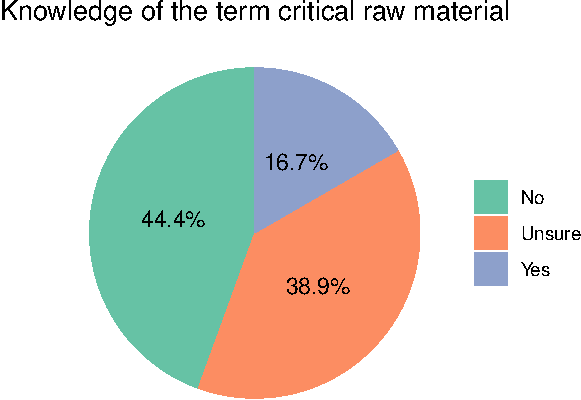
\includegraphics[keepaspectratio]{index_files/figure-pdf/fig-crm-familiarity-1.pdf}}

}

\caption{\label{fig-crm-familiarity}Familiarity of all participants with
the term critical raw material (CRM), before general info was made
available to all, and specific info to a randomized group of the
participants}

\end{figure}%

After that, the survey split into the two groups, hereafter referred to
as the control and the CRM group. The recycling intentions were found to
be very similar for both groups, with no significant difference between
the ones shown the additional info on CRM to the control group. In
Figure~\ref{fig-likert-recycling}, the importance of certain factors in
the case for recycling e-waste showed to be largely unaffected by what
group the respondent was in. Overall, all provided factors were
evaluated similarly to each other, namely as being very to extremely
important. The control group often evaluated reasons to be more
important for recycling e-waste than the CRM group. What's especially
relevant is that they did that also for `reducing dependence on
ethically controversial mining', the main topic of the article shown to
the CRM group.

This allows thus for no statement on the effectiveness or influence of
providing such additional information. It should be mentioned however
that the control group consisted only of 2 participants (CRM group: 14
participants), so its statistical relevance is inexistent in any way.
All provided factors were evaulated similarily to each other.

\begin{Shaded}
\begin{Highlighting}[]
\NormalTok{likert\_recycling }\OtherTok{\textless{}{-}} \FunctionTok{read\_rds}\NormalTok{(}\FunctionTok{here}\NormalTok{(}\StringTok{"data/final/likert\_recycling.rds"}\NormalTok{))}
\NormalTok{likert\_recycling\_long }\OtherTok{\textless{}{-}} \FunctionTok{read\_rds}\NormalTok{(}\FunctionTok{here}\NormalTok{(}\StringTok{"data/final/likert\_recycling\_long.rds"}\NormalTok{))}

\FunctionTok{ggplot}\NormalTok{() }\SpecialCharTok{+}
  \CommentTok{\# Dumbbell layer: from wide{-}format}
  \FunctionTok{geom\_dumbbell}\NormalTok{(}\AttributeTok{data =}\NormalTok{ likert\_recycling,}
                \FunctionTok{aes}\NormalTok{(}\AttributeTok{y =}\NormalTok{ item, }\AttributeTok{x =}\NormalTok{ Control, }\AttributeTok{xend =} \StringTok{\textasciigrave{}}\AttributeTok{CRM mining}\SpecialCharTok{\textbackslash{}n}\AttributeTok{info provided}\StringTok{\textasciigrave{}}\NormalTok{),}
                \AttributeTok{size =} \FloatTok{4.5}\NormalTok{,}
                \AttributeTok{colour =} \StringTok{"gray"}\NormalTok{,}
                \AttributeTok{alpha =} \FloatTok{0.8}\NormalTok{) }\SpecialCharTok{+}
  
  \CommentTok{\# Points layer: from long{-}format}
  \FunctionTok{geom\_point}\NormalTok{(}\AttributeTok{data =}\NormalTok{ likert\_recycling\_long,}
             \FunctionTok{aes}\NormalTok{(}\AttributeTok{x =}\NormalTok{ mean\_score, }\AttributeTok{y =}\NormalTok{ item, }\AttributeTok{color =}\NormalTok{ even\_odd),}
             \AttributeTok{size =} \DecValTok{6}\NormalTok{,}
             \AttributeTok{alpha =} \FloatTok{0.6}\NormalTok{) }\SpecialCharTok{+}
  
  \CommentTok{\# Scale and labels}
  \FunctionTok{scale\_x\_continuous}\NormalTok{(}\AttributeTok{breaks =} \DecValTok{1}\SpecialCharTok{:}\DecValTok{5}\NormalTok{, }\AttributeTok{limits =} \FunctionTok{c}\NormalTok{(}\DecValTok{1}\NormalTok{, }\DecValTok{5}\NormalTok{),}
                     \AttributeTok{labels =} \FunctionTok{c}\NormalTok{(}\StringTok{"(1) Not important at all"}\NormalTok{, }\StringTok{"2"}\NormalTok{, }\StringTok{"3"}\NormalTok{, }\StringTok{"4"}\NormalTok{, }\StringTok{"Extremely important (5)"}\NormalTok{)) }\SpecialCharTok{+}
  \FunctionTok{scale\_color\_manual}\NormalTok{(}\AttributeTok{values =} \FunctionTok{c}\NormalTok{(}\AttributeTok{Control =} \StringTok{"\#0072B2"}\NormalTok{, }\StringTok{\textasciigrave{}}\AttributeTok{CRM mining}\SpecialCharTok{\textbackslash{}n}\AttributeTok{info provided}\StringTok{\textasciigrave{}} \OtherTok{=} \StringTok{"\#D55E00"}\NormalTok{)) }\SpecialCharTok{+}
  \FunctionTok{labs}\NormalTok{(}\AttributeTok{title =} \StringTok{"Reasons for e{-}waste recycling"}\NormalTok{,}
       \AttributeTok{x =} \ConstantTok{NULL}\NormalTok{, }\AttributeTok{y =} \ConstantTok{NULL}\NormalTok{, }\AttributeTok{color =} \StringTok{"Group"}\NormalTok{) }\SpecialCharTok{+}
  \FunctionTok{theme\_minimal}\NormalTok{() }\SpecialCharTok{+}
  \FunctionTok{theme}\NormalTok{(}\AttributeTok{legend.title =} \FunctionTok{element\_text}\NormalTok{(}\AttributeTok{size =} \DecValTok{11}\NormalTok{), }\AttributeTok{legend.text =} \FunctionTok{element\_text}\NormalTok{(}\AttributeTok{size =} \DecValTok{10}\NormalTok{),}
        \AttributeTok{legend.key.size =} \FunctionTok{unit}\NormalTok{(}\FloatTok{0.8}\NormalTok{, }\StringTok{"lines"}\NormalTok{), }\AttributeTok{axis.text.y =} \FunctionTok{element\_text}\NormalTok{(}\AttributeTok{size =} \DecValTok{10}\NormalTok{),}
        \AttributeTok{axis.text.x =} \FunctionTok{element\_text}\NormalTok{(}\AttributeTok{size =} \DecValTok{10}\NormalTok{), }\AttributeTok{plot.title =} \FunctionTok{element\_text}\NormalTok{(}\AttributeTok{size =} \DecValTok{15}\NormalTok{, }\AttributeTok{hjust =} \FloatTok{0.5}\NormalTok{))}
\end{Highlighting}
\end{Shaded}

\begin{figure}[H]

\centering{

\pandocbounded{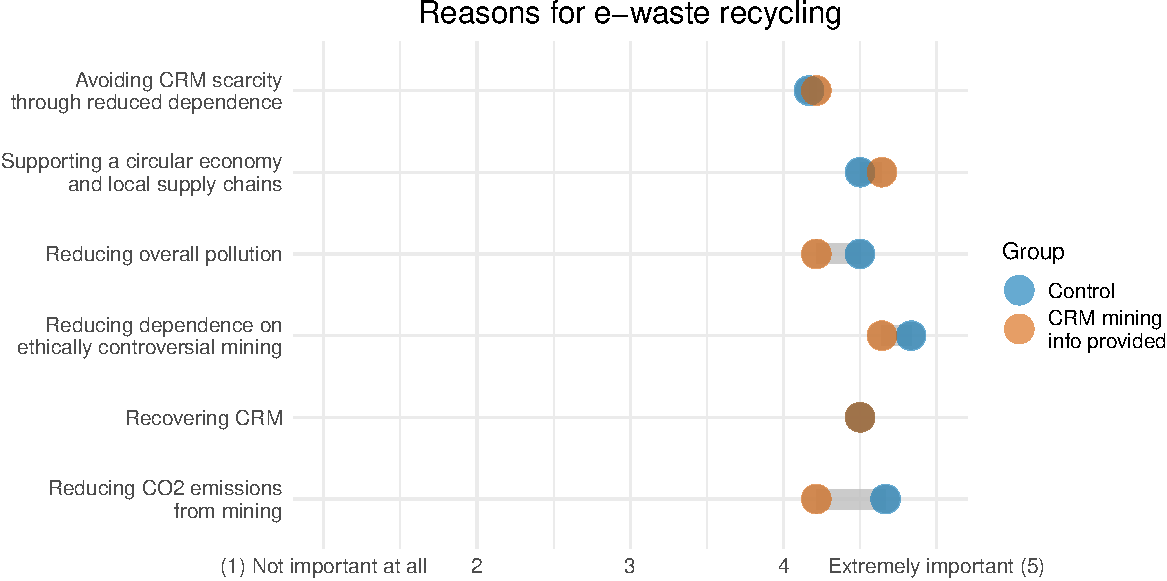
\includegraphics[keepaspectratio]{index_files/figure-pdf/fig-likert-recycling-1.pdf}}

}

\caption{\label{fig-likert-recycling}Contribution of certain factors to
the importance of e-waste recycling, i.e.~how important a factor do you
consider x to be in the case for recycling e-waste?}

\end{figure}%

\begin{Shaded}
\begin{Highlighting}[]
\NormalTok{likert\_intentions }\OtherTok{\textless{}{-}} \FunctionTok{read\_rds}\NormalTok{(}\FunctionTok{here}\NormalTok{(}\StringTok{"data/final/likert\_intentions.rds"}\NormalTok{))}
\NormalTok{likert\_intentions\_long }\OtherTok{\textless{}{-}} \FunctionTok{read\_rds}\NormalTok{(}\FunctionTok{here}\NormalTok{(}\StringTok{"data/final/likert\_intentions\_long.rds"}\NormalTok{))}

\FunctionTok{ggplot}\NormalTok{() }\SpecialCharTok{+}
  \CommentTok{\# Dumbbell layer: from wide{-}format}
  \FunctionTok{geom\_dumbbell}\NormalTok{(}\AttributeTok{data =}\NormalTok{ likert\_intentions,}
                \FunctionTok{aes}\NormalTok{(}\AttributeTok{y =}\NormalTok{ item, }\AttributeTok{x =}\NormalTok{ Control, }\AttributeTok{xend =} \StringTok{\textasciigrave{}}\AttributeTok{CRM mining}\SpecialCharTok{\textbackslash{}n}\AttributeTok{info provided}\StringTok{\textasciigrave{}}\NormalTok{),}
                \AttributeTok{size =} \FloatTok{4.5}\NormalTok{,}
                \AttributeTok{colour =} \StringTok{"gray"}\NormalTok{,}
                \AttributeTok{alpha =} \FloatTok{0.8}\NormalTok{) }\SpecialCharTok{+}
  
  \CommentTok{\# Points layer: from long{-}format}
  \FunctionTok{geom\_point}\NormalTok{(}\AttributeTok{data =}\NormalTok{ likert\_intentions\_long,}
             \FunctionTok{aes}\NormalTok{(}\AttributeTok{x =}\NormalTok{ mean\_score, }\AttributeTok{y =}\NormalTok{ item, }\AttributeTok{color =}\NormalTok{ even\_odd),}
             \AttributeTok{size =} \DecValTok{6}\NormalTok{,}
             \AttributeTok{alpha =} \FloatTok{0.6}\NormalTok{) }\SpecialCharTok{+}
  
  \CommentTok{\# Scale and labels}
  \FunctionTok{scale\_x\_continuous}\NormalTok{(}\AttributeTok{breaks =} \DecValTok{1}\SpecialCharTok{:}\DecValTok{5}\NormalTok{, }\AttributeTok{limits =} \FunctionTok{c}\NormalTok{(}\DecValTok{1}\NormalTok{, }\DecValTok{5}\NormalTok{),}
                     \AttributeTok{labels =} \FunctionTok{c}\NormalTok{(}\StringTok{"(1) Not important at all}\SpecialCharTok{\textbackslash{}n}\StringTok{/very unlikely"}\NormalTok{, }\StringTok{"2"}\NormalTok{, }\StringTok{"3"}\NormalTok{, }\StringTok{"4"}\NormalTok{, }\StringTok{"Extremely important/}\SpecialCharTok{\textbackslash{}n}\StringTok{likely (5)"}\NormalTok{)) }\SpecialCharTok{+}
  \FunctionTok{scale\_color\_manual}\NormalTok{(}\AttributeTok{values =} \FunctionTok{c}\NormalTok{(}\AttributeTok{Control =} \StringTok{"\#0072B2"}\NormalTok{, }\StringTok{\textasciigrave{}}\AttributeTok{CRM mining}\SpecialCharTok{\textbackslash{}n}\AttributeTok{info provided}\StringTok{\textasciigrave{}} \OtherTok{=} \StringTok{"\#D55E00"}\NormalTok{)) }\SpecialCharTok{+}
  \FunctionTok{labs}\NormalTok{(}\AttributeTok{title =} \StringTok{"E{-}waste recycling importance and intentions"}\NormalTok{,}
       \AttributeTok{x =} \ConstantTok{NULL}\NormalTok{, }\AttributeTok{y =} \ConstantTok{NULL}\NormalTok{, }\AttributeTok{color =} \StringTok{"Group"}\NormalTok{) }\SpecialCharTok{+}
  \FunctionTok{theme\_minimal}\NormalTok{() }\SpecialCharTok{+}
  \FunctionTok{theme}\NormalTok{(}\AttributeTok{legend.title =} \FunctionTok{element\_text}\NormalTok{(}\AttributeTok{size =} \DecValTok{11}\NormalTok{), }\AttributeTok{legend.text =} \FunctionTok{element\_text}\NormalTok{(}\AttributeTok{size =} \DecValTok{10}\NormalTok{),}
        \AttributeTok{legend.key.size =} \FunctionTok{unit}\NormalTok{(}\FloatTok{0.8}\NormalTok{, }\StringTok{"lines"}\NormalTok{), }\AttributeTok{axis.text.y =} \FunctionTok{element\_text}\NormalTok{(}\AttributeTok{size =} \DecValTok{10}\NormalTok{),}
        \AttributeTok{axis.text.x =} \FunctionTok{element\_text}\NormalTok{(}\AttributeTok{size =} \DecValTok{10}\NormalTok{), }\AttributeTok{plot.title =} \FunctionTok{element\_text}\NormalTok{(}\AttributeTok{size =} \DecValTok{15}\NormalTok{, }\AttributeTok{hjust =} \FloatTok{0.5}\NormalTok{))}
\end{Highlighting}
\end{Shaded}

\begin{figure}[H]

\centering{

\pandocbounded{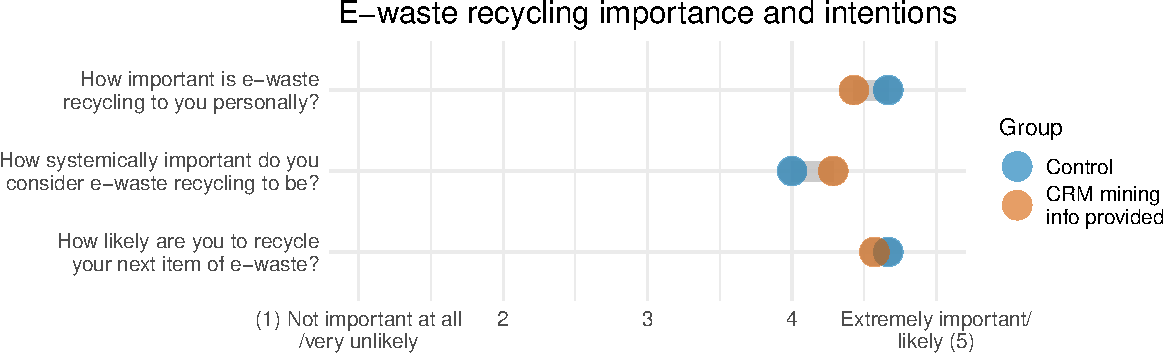
\includegraphics[keepaspectratio]{index_files/figure-pdf/fig-likert-intentions-1.pdf}}

}

\caption{\label{fig-likert-intentions}E-waste recycling intentions and
personal/systemic importance of e-waste recycling.}

\end{figure}%

As seen in Figure~\ref{fig-likert-intentions} and
Figure~\ref{fig-likert-materials}, similar results were found for
overall recycling importance, intentions and when comparing different
materials' recycling. No trend indicating higher importance and
intentions for the CRM groups are recognisable. If anything, it's worth
mentioning that the control group deemed e-waste recycling more
important than the CRM group, but did so with most types of material
recycling, so this could also be attributed to overall higher motivation
to recycle.\\
Nevertheless, recycling intentions are high - very high and personal
importance is weighted a bit higher than systemic importance of
recycling e-waste. The attitudes reflect that the need for recycling,
especially e-waste, is widespread, with metal and PET being evaluated in
a similar fashion, organic waste, paper, cardboard and glass slightly
lower.

\begin{Shaded}
\begin{Highlighting}[]
\NormalTok{likert\_materials }\OtherTok{\textless{}{-}} \FunctionTok{read\_rds}\NormalTok{(}\FunctionTok{here}\NormalTok{(}\StringTok{"data/final/likert\_materials.rds"}\NormalTok{))}
\NormalTok{likert\_materials\_long }\OtherTok{\textless{}{-}} \FunctionTok{read\_rds}\NormalTok{(}\FunctionTok{here}\NormalTok{(}\StringTok{"data/final/likert\_materials\_long.rds"}\NormalTok{))}

\FunctionTok{ggplot}\NormalTok{() }\SpecialCharTok{+}
  \CommentTok{\# Dumbbell layer: from wide{-}format}
  \FunctionTok{geom\_dumbbell}\NormalTok{(}\AttributeTok{data =}\NormalTok{ likert\_materials,}
                \FunctionTok{aes}\NormalTok{(}\AttributeTok{y =}\NormalTok{ item, }\AttributeTok{x =}\NormalTok{ Control, }\AttributeTok{xend =} \StringTok{\textasciigrave{}}\AttributeTok{CRM mining}\SpecialCharTok{\textbackslash{}n}\AttributeTok{info provided}\StringTok{\textasciigrave{}}\NormalTok{),}
                \AttributeTok{size =} \FloatTok{4.5}\NormalTok{,}
                \AttributeTok{colour =} \StringTok{"gray"}\NormalTok{,}
                \AttributeTok{alpha =} \FloatTok{0.8}\NormalTok{) }\SpecialCharTok{+}
  
  \CommentTok{\# Points layer: from long{-}format}
  \FunctionTok{geom\_point}\NormalTok{(}\AttributeTok{data =}\NormalTok{ likert\_materials\_long,}
             \FunctionTok{aes}\NormalTok{(}\AttributeTok{x =}\NormalTok{ mean\_score, }\AttributeTok{y =}\NormalTok{ item, }\AttributeTok{color =}\NormalTok{ even\_odd),}
             \AttributeTok{size =} \DecValTok{6}\NormalTok{,}
             \AttributeTok{alpha =} \FloatTok{0.6}\NormalTok{) }\SpecialCharTok{+}
  
  \CommentTok{\# Scale and labels}
  \FunctionTok{scale\_x\_continuous}\NormalTok{(}\AttributeTok{breaks =} \DecValTok{1}\SpecialCharTok{:}\DecValTok{5}\NormalTok{, }\AttributeTok{limits =} \FunctionTok{c}\NormalTok{(}\DecValTok{1}\NormalTok{, }\DecValTok{5}\NormalTok{),}
                     \AttributeTok{labels =} \FunctionTok{c}\NormalTok{(}\StringTok{"(1) Not important at all"}\NormalTok{, }\StringTok{"2"}\NormalTok{, }\StringTok{"3"}\NormalTok{, }\StringTok{"4"}\NormalTok{, }\StringTok{"Extremely important (5)"}\NormalTok{)) }\SpecialCharTok{+}
  \FunctionTok{scale\_color\_manual}\NormalTok{(}\AttributeTok{values =} \FunctionTok{c}\NormalTok{(}\AttributeTok{Control =} \StringTok{"\#0072B2"}\NormalTok{, }\StringTok{\textasciigrave{}}\AttributeTok{CRM mining}\SpecialCharTok{\textbackslash{}n}\AttributeTok{info provided}\StringTok{\textasciigrave{}} \OtherTok{=} \StringTok{"\#D55E00"}\NormalTok{)) }\SpecialCharTok{+}
  \FunctionTok{labs}\NormalTok{(}\AttributeTok{title =} \StringTok{"Importance of selected materials recycling"}\NormalTok{,}
       \AttributeTok{subtitle =} \StringTok{"How important do participants consider the recycling of the following materials to be?"}\NormalTok{,}
       \AttributeTok{x =} \ConstantTok{NULL}\NormalTok{, }\AttributeTok{y =} \ConstantTok{NULL}\NormalTok{, }\AttributeTok{color =} \StringTok{"Group"}\NormalTok{) }\SpecialCharTok{+}
  \FunctionTok{theme\_minimal}\NormalTok{() }\SpecialCharTok{+}
  \FunctionTok{theme}\NormalTok{(}\AttributeTok{legend.title =} \FunctionTok{element\_text}\NormalTok{(}\AttributeTok{size =} \DecValTok{11}\NormalTok{), }\AttributeTok{legend.text =} \FunctionTok{element\_text}\NormalTok{(}\AttributeTok{size =} \DecValTok{10}\NormalTok{),}
        \AttributeTok{legend.key.size =} \FunctionTok{unit}\NormalTok{(}\FloatTok{0.8}\NormalTok{, }\StringTok{"lines"}\NormalTok{), }\AttributeTok{axis.text.y =} \FunctionTok{element\_text}\NormalTok{(}\AttributeTok{size =} \DecValTok{10}\NormalTok{),}
        \AttributeTok{axis.text.x =} \FunctionTok{element\_text}\NormalTok{(}\AttributeTok{size =} \DecValTok{10}\NormalTok{), }\AttributeTok{plot.title =} \FunctionTok{element\_text}\NormalTok{(}\AttributeTok{size =} \DecValTok{15}\NormalTok{, }\AttributeTok{hjust =} \FloatTok{0.5}\NormalTok{))}
\end{Highlighting}
\end{Shaded}

\begin{figure}[H]

\centering{

\pandocbounded{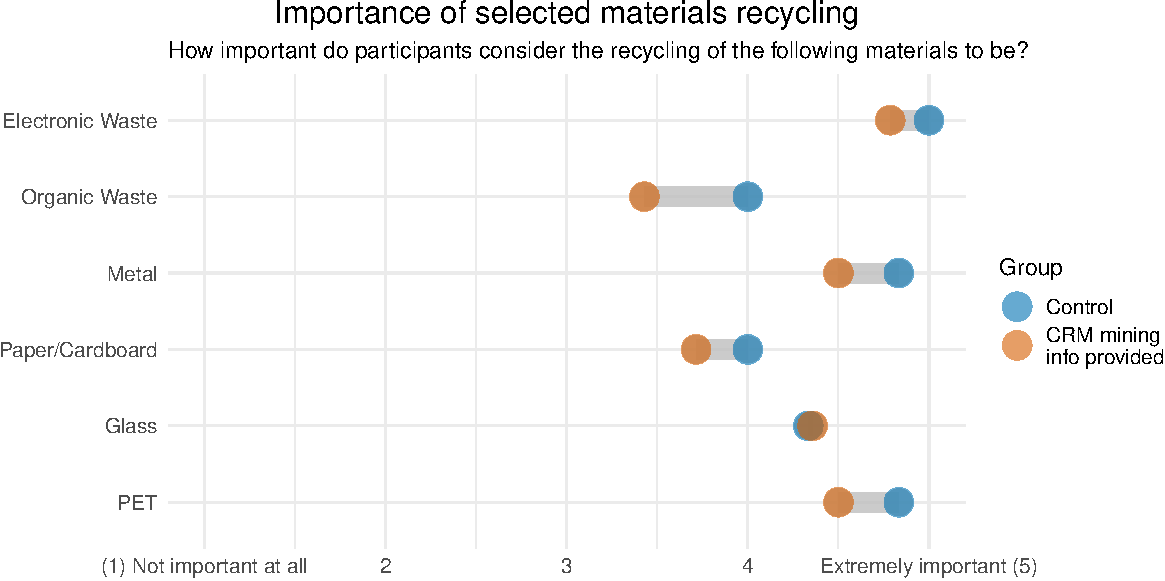
\includegraphics[keepaspectratio]{index_files/figure-pdf/fig-likert-materials-1.pdf}}

}

\caption{\label{fig-likert-materials}Subjective relevance of the
recycling of selected materials of which recycling is readily available
in CH.}

\end{figure}%

A visualization of the demographics of the survey's participants can be
seen in the Appendix, Figure~\ref{fig-demographics}.

\section{Conclusion}\label{conclusion}

\begin{itemize}
\item
  Recycling intentions and attitudes towards e-waste are very high among
  the survey's respondents, mainly young, highly educated people living
  in shared apartments.
\item
  Including targeted information on CRM and its ethically controversial
  sourcing in countries like the DRC did not show any significant effect
  on e-waste recycling intentions and attitudes.
\item
  This is mainly attributed to the statistically insignificant amount of
  responses of either group and the high education level of
  participants.
\end{itemize}

\section{Appendix}\label{appendix}

\subsection{Additional Figures}\label{additional-figures}

\begin{Shaded}
\begin{Highlighting}[]
\NormalTok{household\_data }\OtherTok{\textless{}{-}} \FunctionTok{read\_csv}\NormalTok{(}\FunctionTok{here}\NormalTok{(}\StringTok{"data/final/household.csv"}\NormalTok{), }\AttributeTok{show\_col\_types =} \ConstantTok{FALSE}\NormalTok{)}
\NormalTok{education\_data }\OtherTok{\textless{}{-}} \FunctionTok{read\_csv}\NormalTok{(}\FunctionTok{here}\NormalTok{(}\StringTok{"data/final/education.csv"}\NormalTok{), }\AttributeTok{show\_col\_types =} \ConstantTok{FALSE}\NormalTok{)}

\NormalTok{plot1 }\OtherTok{\textless{}{-}} \FunctionTok{ggplot}\NormalTok{(education\_data, }\FunctionTok{aes}\NormalTok{(}\AttributeTok{x =} \StringTok{""}\NormalTok{, }\AttributeTok{y =}\NormalTok{ n, }\AttributeTok{fill =}\NormalTok{ degree)) }\SpecialCharTok{+}
  \FunctionTok{geom\_col}\NormalTok{(}\AttributeTok{width =} \DecValTok{1}\NormalTok{) }\SpecialCharTok{+}
  \FunctionTok{coord\_polar}\NormalTok{(}\AttributeTok{theta =} \StringTok{"y"}\NormalTok{) }\SpecialCharTok{+}
  \FunctionTok{geom\_text}\NormalTok{(}\FunctionTok{aes}\NormalTok{(}\AttributeTok{label =} \FunctionTok{paste0}\NormalTok{(percentage, }\StringTok{"\%"}\NormalTok{)),}
            \AttributeTok{position =} \FunctionTok{position\_stack}\NormalTok{(}\AttributeTok{vjust =} \FloatTok{0.5}\NormalTok{),}
            \AttributeTok{size =} \DecValTok{4}\NormalTok{) }\SpecialCharTok{+}
  \FunctionTok{scale\_fill\_brewer}\NormalTok{(}\AttributeTok{palette =} \StringTok{"Set2"}\NormalTok{) }\SpecialCharTok{+}
  \FunctionTok{theme\_void}\NormalTok{() }\SpecialCharTok{+}
  \FunctionTok{labs}\NormalTok{(}\AttributeTok{title =} \StringTok{"Highest completed degree of participants"}\NormalTok{) }\SpecialCharTok{+} 
  \FunctionTok{theme}\NormalTok{(}\AttributeTok{legend.title =} \FunctionTok{element\_blank}\NormalTok{())}

\NormalTok{plot2 }\OtherTok{\textless{}{-}} \FunctionTok{ggplot}\NormalTok{(household\_data, }\FunctionTok{aes}\NormalTok{(}\AttributeTok{x =} \StringTok{""}\NormalTok{, }\AttributeTok{y =}\NormalTok{ n, }\AttributeTok{fill =}\NormalTok{ household)) }\SpecialCharTok{+}
  \FunctionTok{geom\_col}\NormalTok{(}\AttributeTok{width =} \DecValTok{1}\NormalTok{) }\SpecialCharTok{+}
  \FunctionTok{coord\_polar}\NormalTok{(}\AttributeTok{theta =} \StringTok{"y"}\NormalTok{) }\SpecialCharTok{+}
  \FunctionTok{geom\_text}\NormalTok{(}\FunctionTok{aes}\NormalTok{(}\AttributeTok{label =} \FunctionTok{paste0}\NormalTok{(percentage, }\StringTok{"\%"}\NormalTok{)),}
            \AttributeTok{position =} \FunctionTok{position\_stack}\NormalTok{(}\AttributeTok{vjust =} \FloatTok{0.5}\NormalTok{),}
            \AttributeTok{size =} \DecValTok{4}\NormalTok{) }\SpecialCharTok{+}
  \FunctionTok{scale\_fill\_brewer}\NormalTok{(}\AttributeTok{palette =} \StringTok{"Set2"}\NormalTok{) }\SpecialCharTok{+}
  \FunctionTok{theme\_void}\NormalTok{() }\SpecialCharTok{+}
  \FunctionTok{labs}\NormalTok{(}\AttributeTok{title =} \StringTok{"Household type of participants"}\NormalTok{) }\SpecialCharTok{+} 
  \FunctionTok{theme}\NormalTok{(}\AttributeTok{legend.title =} \FunctionTok{element\_blank}\NormalTok{(), }\AttributeTok{plot.title =} \FunctionTok{element\_text}\NormalTok{(}\AttributeTok{hjust =} \FloatTok{0.5}\NormalTok{))}

\NormalTok{plot1 }\SpecialCharTok{+}\NormalTok{ plot2}
\end{Highlighting}
\end{Shaded}

\begin{figure}[H]

\centering{

\pandocbounded{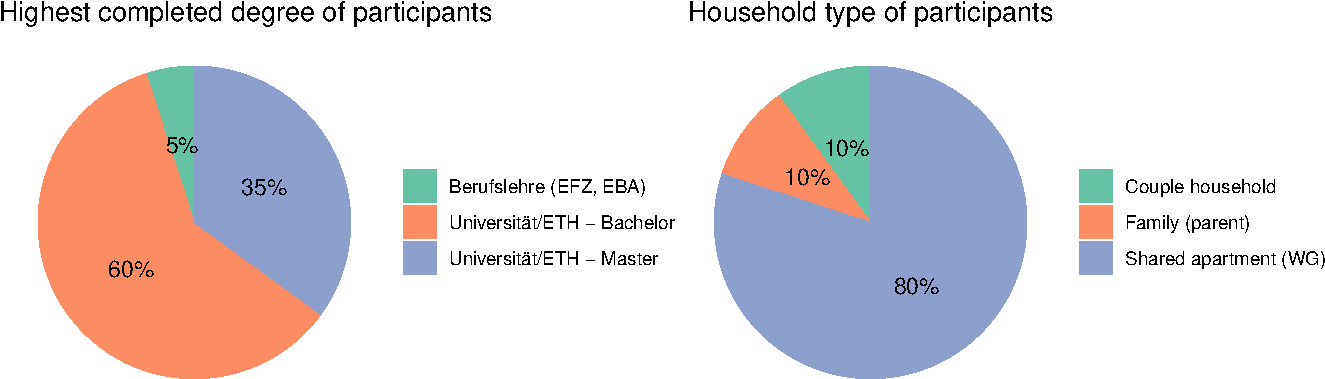
\includegraphics[keepaspectratio]{index_files/figure-pdf/fig-demographics-1.pdf}}

}

\caption{\label{fig-demographics}Demographic info on the participants}

\end{figure}%

\phantomsection\label{refs}
\begin{CSLReferences}{1}{0}
\bibitem[\citeproctext]{ref-cucchiella2015recycling}
Cucchiella, Federica, Idiano D'Adamo, S. C. Lenny Koh, and Paolo Rosa.
2015. {``Recycling of {WEEEs}: {An} Economic Assessment of Present and
Future e-Waste Streams.''} \emph{Renewable and Sustainable Energy
Reviews} 51 (November): 263--72.
\url{https://doi.org/10.1016/j.rser.2015.06.010}.

\bibitem[\citeproctext]{ref-european}
{``European {Critical Raw Materials Act} - {European Commission}.''}
2023.
https://commission.europa.eu/strategy-and-policy/priorities-2019-2024/european-green-deal/green-deal-industrial-plan/european-critical-raw-materials-act\_en.

\bibitem[\citeproctext]{ref-heacock2016ewaste}
Heacock, Michelle, Carol Bain Kelly, Kwadwo Ansong Asante, Linda S.
Birnbaum, Åke Lennart Bergman, Marie-Noel Bruné, Irena Buka, et al.
2016. {``E-{Waste} and {Harm} to {Vulnerable Populations}: {A Growing
Global Problem}.''} \emph{Environmental Health Perspectives} 124 (5):
550--55. \url{https://doi.org/10.1289/ehp.1509699}.

\bibitem[\citeproctext]{ref-ethical}
Huff, Michael. 2023. {``Ethical Cobalt Mining Is Critical to Electronic
Markets.''} \emph{Electronics360.globalspec.com}.
https://electronics360.globalspec.com/article/19457/ethical-cobalt-mining-is-critical-to-electronic-markets.

\bibitem[\citeproctext]{ref-liu2023global}
Liu, Kang, Quanyin Tan, Jiadong Yu, and Mengmeng Wang. 2023. {``A Global
Perspective on e-Waste Recycling.''} \emph{Circular Economy} 2 (1):
100028. \url{https://doi.org/10.1016/j.cec.2023.100028}.

\bibitem[\citeproctext]{ref-perkins2014ewaste}
Perkins, Devin N., Marie-Noel Brune Drisse, Tapiwa Nxele, and Peter D.
Sly. 2014. {``E-{Waste}: {A Global Hazard}.''} \emph{Annals of Global
Health} 80 (4): 286--95.
\url{https://doi.org/10.1016/j.aogh.2014.10.001}.

\end{CSLReferences}




\end{document}
